\documentclass[conference]{IEEEtran}
\usepackage{blindtext, graphicx}

\usepackage[slovak]{babel}
\usepackage[utf8]{inputenc}
\usepackage{cite}

% correct bad hyphenation here
\hyphenation{op-tical net-works semi-conduc-tor}

\begin{document}
%
% paper title
% can use linebreaks \\ within to get better formatting as desired
\title{Implementácia modifikovaného algoritmu SHA-1 v jazyku C (CPU) a CUDA (GPU)}

% author names and affiliations
% use a multiple column layout for up to three different
% affiliations
\author{\IEEEauthorblockN{Peter Kaňuch}
\IEEEauthorblockA{Fakulta informatiky a informačných technológií\\
Slovenská Technická Univerzita\\
Slovenská republika, Bratislava\\
Email: xkanuch@stuba.sk}}

% use for special paper notices
%\IEEEspecialpapernotice{(Invited Paper)}

% make the title area
\maketitle

\begin{abstract}
%\boldmath

\end{abstract}


\begin{IEEEkeywords}
IEEEtran, journal, \LaTeX, paper, template.
\end{IEEEkeywords}


\IEEEpeerreviewmaketitle


\section{Úvod}

\section{CPU verzus GPU architektúra}

\subsection{Architektúra počítačových procesorov}

CPU (Central Processing Unit) alebo aj procesor, je hlavný komponent počítača, ktorý načítava, spracováva a vykonáva inštrukcie nad rôznymi dátami. Procesor pozostáva z dvoch hlavných častí:

\begin{itemize}
	\item{kontrolná jednotka (CU)}
	\item{aritmeticko-logická jednotka (ALU)}
\end{itemize}

Základný procesor pozostáva z piatich fáz \cite{hennessy2007compute}: 

\begin{itemize}
	\item{FETCH - fáza, v ktorej sa načítava inštrukcia z pamäte do procesora na základe adresy v registry IP/PC (instruction pointer/program counter) a jeho následnej inkrementácii na ďalšiu adresu }
	\item{DECODE - zabezpečuje dekódovanie inštrukcie}
	\item{EXECUTE - fáza, v ktorej procesor vykonáva rôzne výpočty pomocou ALU}
	\item{MEM (Memory Access) - v tejto fáze, procesor pristupuje do pamäte pre načítanie alebo uloženie dát}
	\item{WB (Write Back) - procesor zapíše výsledky(hodnoty z predošlých fáz vypočítané v ALU) alebo hodnoty načítané z pamäte v predchádzajúcej fáze do registrov}
\end{itemize}

\begin{figure}[!h]
\centering
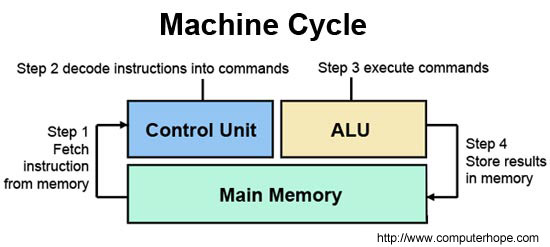
\includegraphics[width=4in]{img/CPU-cycle}
\caption{Základný cyklus procesora}
\end{figure}

Takáto základná architektúra bola postupne vylepšovaná rôznymi mechanizmami (prúdovým spracovaním, detekciou a riešením hazardov, predikciou vetvenia a iné) pre dosiahnutie čo najlepšieho výkonu, t.j. dosiahnutie čo najmenšieho CPI (CPI - počet cyklov na inštrukciu).




\subsection{Architektúra grafických procesorov}

\section{Opis riešenia}

\subsection{Algoritmus SHA-1 a jeho modifikácia}

\subsection{Testovacie prostredie a implementácia}

\section{Výsledky a grafické porovnanie}

\section{Záver}


\appendices
\section{aaa}



% use section* for acknowledgement
\section*{Acknowledgment}


The authors would like to thank...


% Can use something like this to put references on a page
% by themselves when using endfloat and the captionsoff option.
\ifCLASSOPTIONcaptionsoff
  \newpage
\fi




\begin{thebibliography}{1}

\bibitem{hennessy2007compute}
HENNESSY, John L.; PATTERSON, David A. Computer architecture: a quantitative approach. Elsevier, 2007.

\bibitem{tatourian}
TATOURIAN, Alan. Nvidia gpu architecture and cuda programming environment. URL http://code. msdn. microsoft. com/windowsapps/NVIDIA-GPU-Architecture-45c11e6d, 2013.

\end{thebibliography}






\end{document}


